\chapter{Design}\label{ch:design}

\section{CoinMarketCap}\label{sec:coinmarketcap}
some intro
\section{Overview}
\begin{figure}[ht]
    \centering
    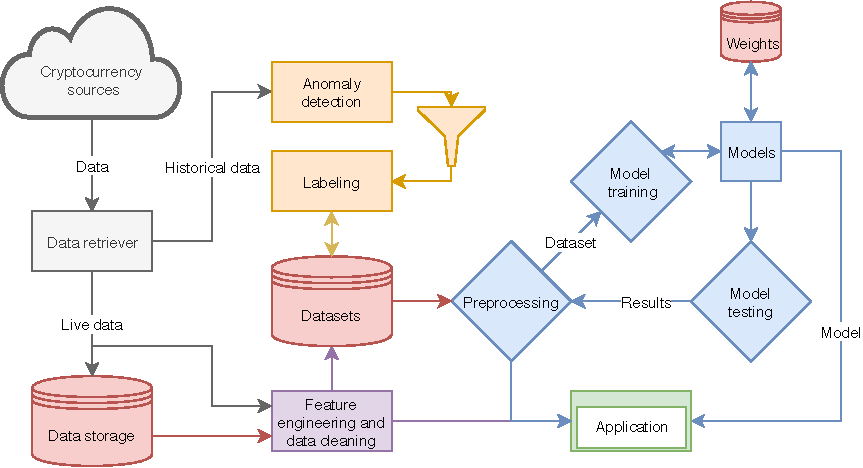
\includegraphics[width=\textwidth]{overview.pdf}
    \caption{Architectural overview}
    \label{fig:overview}
\end{figure}

\section{Data Storage}
% intro
% which exchange to extract data from 
% BTC market
% ohlcv, depth
% csv
% writing every n second
% describe features
%
\subsection{Select exchanges}

\href{https://www.cryptopia.co.nz/}{Cryptopia} suffered a security breach January 14, 2019~\cite{cryptopia_breach_2} and was forced to shut down for a period as the breach also led to an investigation by the New Zealand Police~\cite{cryptopia_breach_1}, the law enforcement says they were acquainted with potentially unauthorized transaction activity of significant amount of cryptocurrency. Cryptopia later announced on twitter Mars 18, 2019 that they "completed their maintenance and the site is back up.", Nevertheless, we are still a bit skeptical and choose to avoid Cryptopia.

\href{https://yobit.net/en/}{Yobit} to all surprise and on multiple occasions has announced through their official Twitter account with over 160 thousand followers~\cite{yobit_twitter}, that they are launching a coin-pump on a random coin. They even have a countdown timer on their web-page for signalizing when the coin-pump starts. In addition, various platforms are accusing Yobit of selling fake coins~\cite{yobit_fake_1, yobit_fake_2, yobit_fake_3}, which are most likely to be true when they have over four thousand different symbol-pairs in their Bitcoin market~\cite{yobit_market}, while there are only slightly over two thousand cryptocurrencies in existence according to CoinMarketCap. We believe that Yobit has the elements of a casino where the house always wins and choosing not to play them on their own game, and collecting artificial coin-pumps organized by Yobit may cause noise in the dataset as it necessarily do not reflect a \ac{pd}.

\begin{figure}[ht]
    \centering
    
\includegraphics[width=\textwidth]{yobit.pdf}
    \caption{Yobit announcing a coin-pump through their official Twitter account}
    \label{fig:yobit}
\end{figure}

Bittrex banning all \ac{pd} from December ...

% kraken???

% Binance


\subsection{Features Description}
\begin{table}[ht]
    \centering
    \begin{tabular}{p{0.30\textwidth} p{0.70\textwidth}}
        \hline
        \textbf{Feature} & \textbf{Description}\\
        \hline
        \ac{ohlcv}                      & Latest \ac{ohlcv} values.\\
        \hline
        \ac{ohlcv} multiple exchanges   & Aggregated \ac{ohlcv} values from multiple exchanges.\\
        \hline
        Order book                      & Level $1$ (aggregated price and volume) order book with a depth of $5$.\\
        \hline
        Order book imbalance            & The imbalance between bids and asks orders and quantity.\\
        \hline
        Coin capitalization ratio       & Coin capitalization ratio.\\
        \hline
        Volume traded                   & Base and quote volume traded for the last $24$ hours.\\
        \hline
        number of trades                & Number of completed trades for the last $24$ hours.\\      
        \hline
        bid and ask price               & Best bid and ask price for the last $24$ hours.\\
        \hline
        bid and ask volume              & Best bid and ask quantity for the last $24$ hours.\\
        \hline
        Average price                   & Average price for the last $24$ hours.\\
        \hline
        symbol-pair exchange rate       & The rate of how many exchanges that lists the symbol-pair.\\ 
        \hline
        Time                            & Unix timestamp.\\
        \hline
    \end{tabular}
    \caption[Features description]{Feature description}
    \label{tab:features}
\end{table}



\newpage
\section{Data Processing}
% intro

\begin{figure}[ht]
    \centering
    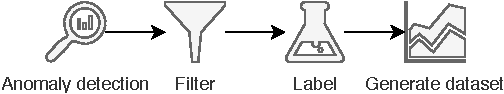
\includegraphics{data_processing.pdf}
    \caption{Data processing pipeline}
    \label{fig:data_processing}
\end{figure}

% hand-picking - infeasible
\subsection{Anomaly Detection}
Manually collecting \ac{pd} events from chat applications to train a \ac{ml} model, seems infeasible in the long run — even tough Livshits and Xu [30] hand-picked $220$ pump-events from July to November in 2018 from $358$ different Telegram groups to train a Random Forest. They still did miss out on plenty of other executed \ac{pd} schemes as there are numerous of other chatting applications and private channels~\cite{blockonomi}. Also, searching for \ac{pd} events is a time-consuming process, and incorrect labeling of \ac{pd} schemes occurs when we lack membership to all of \ac{pd} groups, which results in poorer prediction performance of any \ac{ml} model~\cite{label_noise}. Instead, we believe that it is possible to hand-pick \acp{pd} by \emph{reasoning abductively} with the help of an anomaly detection algorithm to pinpoint suspicious time intervals in historical data.
% ADD - pumps can also fail!  
%

% time window
Before laying out the anomaly detection algorithm, we need to understand \emph{sliding time windows}. A sliding window is a period that stretches back in time (lag factor) from the present containing events at certain intervals. The event intervals can overlap with each other as \autoref{fig:timewindow} illustrates or they can be disjunct. As events exceed the lag factor, they fall out of the sliding window, and they are no longer matching against the rules applied to the sliding window~\cite{redhat}. With a sliding window, we can compare values in a given period~\cite{P&D_to_the_moon}, contrary to using single values, which not yielding much information alone in a timeline. 
\begin{figure}[ht]
    \centering
    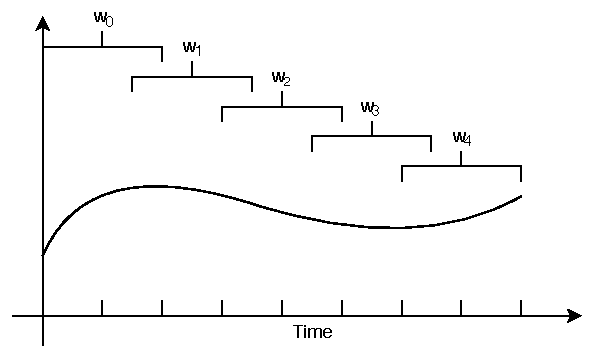
\includegraphics{timewindow.pdf}
    \caption{Sliding time window}
    \label{fig:timewindow}
\end{figure}

% Anomaly detection
The anomaly detection algorithm is proposed by Kleinberg and Kamps \cite{P&D_to_the_moon}, which is inspired by previous research in \ac{dos} attacks~\cite{dos}. It is a threshold based technique to find suspicious value increases in trading price and volume of a symbol-pair. If the price and volume in a specific interval are greater than some threshold, then the interval is flagged anomalous and worth further investigation.

\subsubsection{Price Anomaly}
We compute the price anomaly threshold by a simple moving average $\mu_\gamma^p$ of \ac{ohlcv} values denoted $x$ with a lag factor $\gamma$ multiplied with a given percentage increase $\epsilon_p$. We consider $x$ and $\gamma$ as \ac{ohlcv} objects, and $x-\gamma$ indicates moving backwards in the sliding time window by a factor of $\gamma$~\cite{P&D_to_the_moon}. If the highest registered price in $x$'s time period are greater than the computed threshold, we flag the period as anomalous.
\begin{align}
    \mu_\gamma^p(x) &= \frac{\sum^x_{i=x-\gamma} x_{close}}{\gamma}\\
    price\_anomaly(x)&=
    \begin{cases}
        True  & \text{if $x_{high} >    \epsilon_p \cdot \mu_\gamma^p(x)$}\\
        False & \text{otherwise}
    \end{cases}
\end{align}

\subsubsection{Volume Anomaly}
Calculating the volume anomaly threshold is almost identical to the above, we are only substituting $x_{closing}$ and $x_{high}$ with $x_{volume}$, resulting in.  
\begin{align*}
    \mu_\gamma^v(x) &= \frac{\sum^x_{i=x-\gamma} x_{volume}}{\gamma}\\
    volume\_anomaly(x)&=
    \begin{cases}
        True  & \text{if $x_{volume} >    \epsilon_v \cdot \mu_\gamma^v(x)$}\\
        False & \text{otherwise}
    \end{cases}
\end{align*}
\myequations{Anomaly - Volume}

\subsection{Pump-and-Dump Selection}
% plot - ohlc flagged intervals
% check reinforcers

\subsection{Labeling}

\subsection{Generating a normalized dataset}
% general model
% how we normalize vectors
% lag - number of events in the timeframe

\section{Model Training}
% normalization of data
% training

\section{Deployment}
% sell if pd
% possible to buy before?
% train the model after it is deployed